\documentclass[12pt,a4paper]{article}

\usepackage[utf8]{inputenc}
\usepackage[T1]{fontenc}
\usepackage[swedish]{babel}
\usepackage{amsmath}
\usepackage{ae}
\usepackage{units}
\usepackage{icomma}
\usepackage{color}
\usepackage{graphicx}
\usepackage{bbm}
\newcommand{\N}{\ensuremath{\mathbbm{N}}}
\newcommand{\Z}{\ensuremath{\mathbbm{Z}}}
\newcommand{\Q}{\ensuremath{\mathbbm{Q}}}
\newcommand{\R}{\ensuremath{\mathbbm{R}}}
\newcommand{\C}{\ensuremath{\mathbbm{C}}}
\newcommand{\rd}{\ensuremath{\mathrm{d}}}
\newcommand{\id}{\ensuremath{\,\rd}}


\begin{document}

\title{Simulations of road blockages, Simulation of complex systems}
\author{Fredrik, Daniel, Thorben, Atonderski}
\date{\today}
\maketitle

\begin{abstract}
In real-world traffic small errors, like an unnecessary brake from individual drivers can propagate through traffic and lead to interruptions and traffic jams far away from the initial disturbance. Studying these phenomena could be especially important with the emergence of self-driving cars. The cars need to be tuned so they don't cause unnecessary traffic congestion.

We want to study how small irregularites, such as braking or acceleration of a few drivers, in traffic flow propagate through traffic. We start from a single lane situation with agent-based modelling of individual drivers and periodic boundary condidtions. Each agent is represented by a finite-state machine with threes states, braking, acceleration and driving at constant speed. The state transitions depend on the speed and positions of the nearest neighbours, primarily the one ahead. Depending on the time available, more complexity will be added to the model.  

main features to be implemented:
Graphics - matplotlib/pygame,
Track - linked list, keep track of length, be able to give info to car.
Car - properties: speed, positions, (lane?), state (braking, acceleration, constant), (size?). Functions: update(), query track.
Braking - instantly
Crashes, not in the beginning
Main controller


\end{abstract}

\newpage
\tableofcontents
\newpage

\section{So far, i.e. predraft}
So far we've implemented a rudimentary model of the car track, with regular and more agressive drivers and a visualization. We have also started implementing a basic density plot in order to see the propagation and or creation and dissipation of traffic congestions on the track. So far we have observed wave-like behaviour of car/speeds. Further work will concentrate on extending the model to multi-lane, and extracting the wave propagation-speed/amplitudes etc and their dependence on the number of drivers on the track and the ratio of normal/aggressive drivers and number of lanes etc



\section{The model}

\section{Results}

\begin{figure}[h]
    \centering
    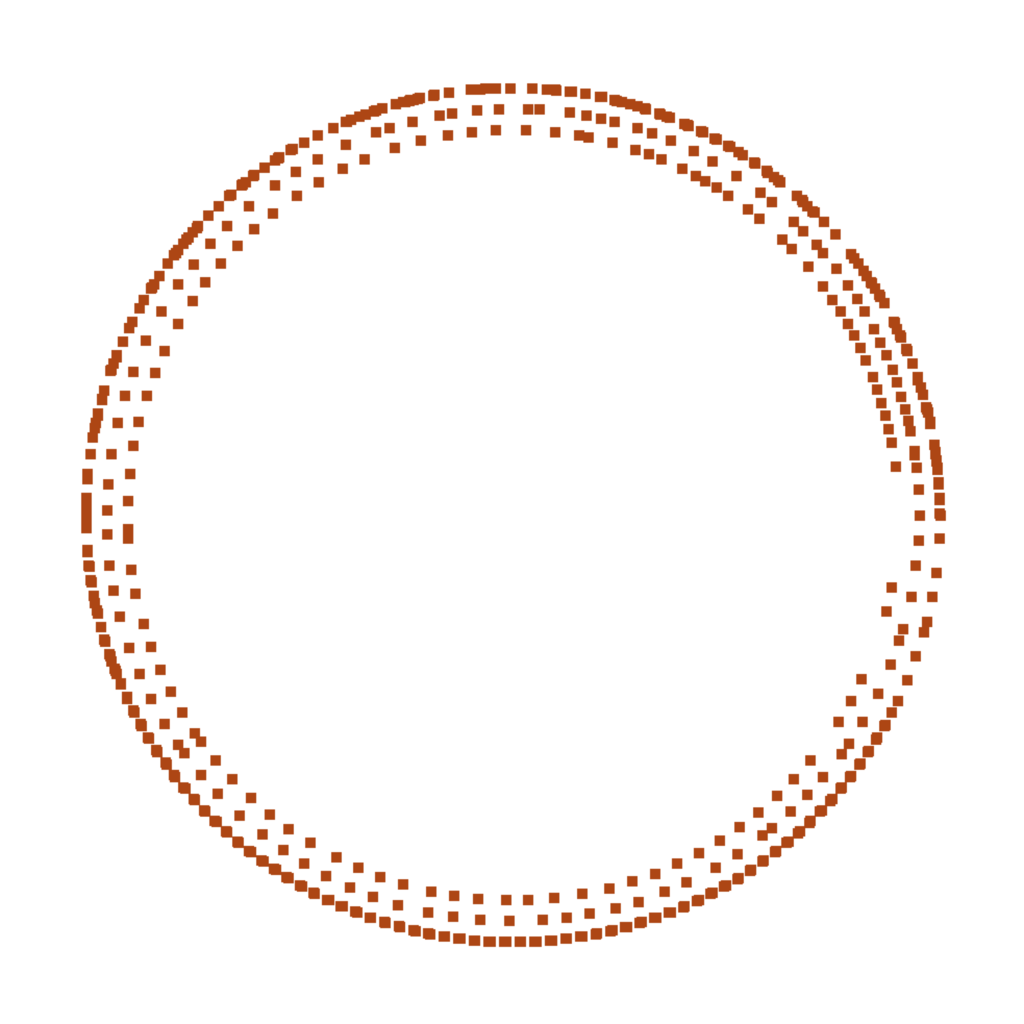
\includegraphics[scale=0.3]{figs/circular_three_lane.png}
    \caption{3 lanes}
    \label{fig:3lanes}
\end{figure}

\begin{figure}[h]     
    \centering
      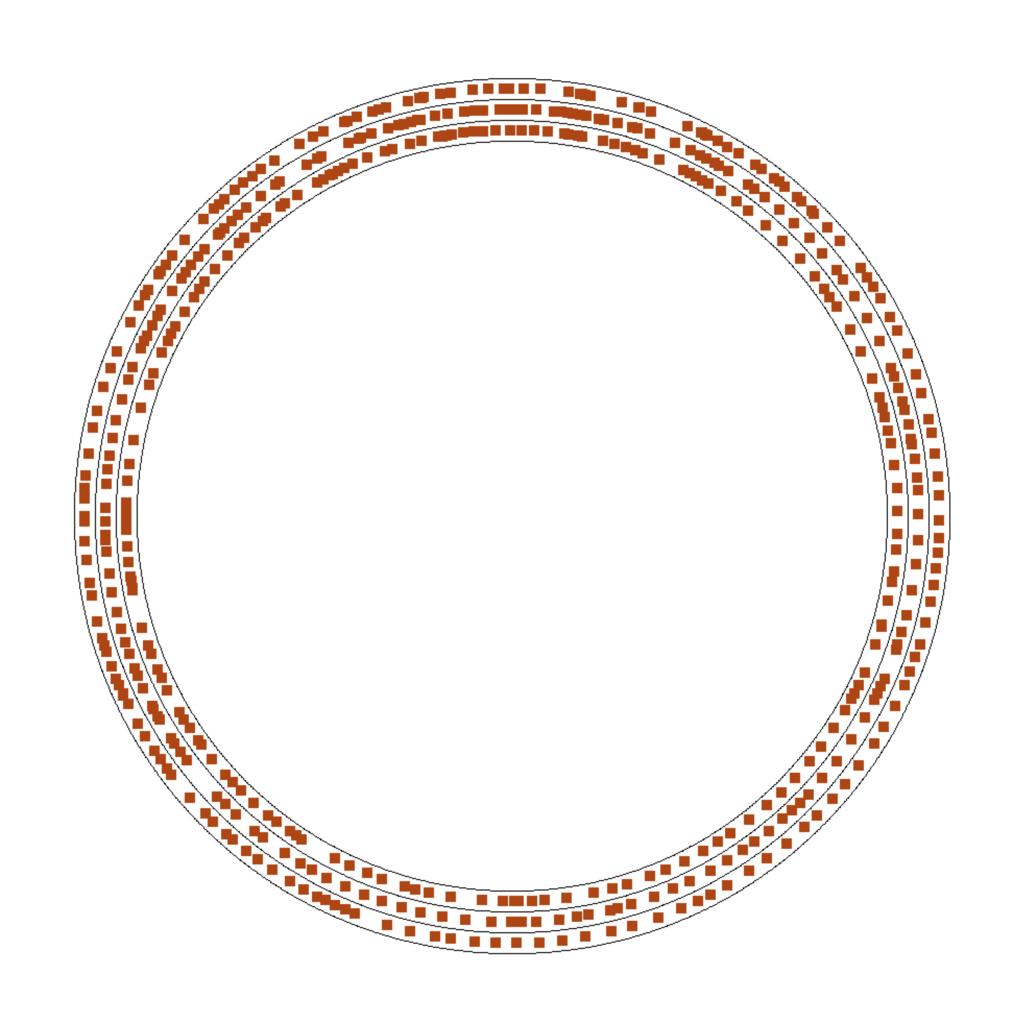
\includegraphics[scale=0.3]{figs/good_circular_three_lane.png}
      \caption{3 lanes}
      \label{fig:3lanes}
\end{figure}

\section{Parameter dependence of cluster formations etc...}

\subsection{}

% Figurer inkluderade som eps-filer
%% \begin{figure}\centering
%% \includegraphics{filnamn.eps}
%% \caption{\label{figuren} Perioden $T$ som funktion av pendellängden.}
%% \end{figure}

% Figurer inkluderade med xfigs postscript+latex
%% \begin{figure}\centering
%% \input{filnamn.pstex_t}
%% \caption{\label{finafiguren} Perioden $T$ som funktion av
%%   pendellängden.}
%% \end{figure}

\end{document}
